\documentclass[12pt]{article}
\usepackage{microtype}

% The preceding line is only needed to identify funding in the first footnote. If that is unneeded, please comment it out.
\usepackage{amsmath,amssymb,amsfonts}
\usepackage{algorithmic}
\usepackage{graphicx}
\usepackage{textcomp}
\usepackage{xcolor}
\usepackage{url}
\usepackage{listings}
\usepackage{courier}
\usepackage{xspace}
\usepackage{multirow}
\usepackage{colortbl}
\usepackage{blindtext}
\usepackage{float}
\usepackage{hyperref}
%\usepackage[font=scriptsize]{caption}
%\newcommand{\sd}[1]{\textbf{"\textsc{SD:}} \textit{#1}"}
%Dessin
\usepackage{tikz}
\usepackage{verbatim}
\usepackage{graphicx}
\usepackage[utf8]{inputenc}
\usepackage[english]{babel}
\usepackage{subfigure}
 \newboolean{showcomments}
\setboolean{showcomments}{true}
\ifthenelse{\boolean{showcomments}}
  {\newcommand{\bnote}[2]{
	\fbox{\bfseries\sffamily\scriptsize#1}
    {\sf\small$\blacktriangleright$\textit{#2}$\blacktriangleleft$}
    % \marginpar{\fbox{\bfseries\sffamily#1}}
   }
   \newcommand{\cvsversion}{\emph{\scriptsize$-$Id: macros.tex,v 1.1.1.1 2007/02/28 13:43:36 bergel Exp $-$}}
  }
  {\newcommand{\bnote}[2]{}
   \newcommand{\cvsversion}{}
  } 


\newcommand{\here}{\bnote{***}{CONTINUE HERE}}
\newcommand{\nb}[1]{\bnote{NB}{#1}}

\newcommand{\fix}[1]{\bnote{FIX}{#1}}
%%%% add your own macros 


\newcommand{\an}[1]{\bnote{Anne}{#1}}
\newcommand{\sd}[1]{\bnote{Stef}{#1}}
\newcommand{\ja}[1]{\bnote{Jannik}{#1}}
\newcommand{\md}[1]{\bnote{MD}{#1}}
\newcommand{\caro}[1]{\bnote{Caro}{#1}}
\newcommand{\jr}[1]{\bnote{JRe}{#1}}
\newcommand{\lf}[1]{\bnote{Luc}{#1}}
\newcommand{\gp}[1]{\bnote{Guille}{#1}}
\newcommand{\pt}[1]{\bnote{Pablo}{#1}}
\newcommand{\theo}[1]{\bnote{Theo}{#1}}
\newcommand{\spb}[1]{\bnote{Santiago}{#1}}
\newcommand{\bv}[1]{\bnote{Beno\^{i}t}{#1}}

\graphicspath{{figures/}}
%%% 


\newcommand{\figref}[1]{Figure~\ref{fig:#1}}
\newcommand{\figlabel}[1]{\label{fig:#1}}
\newcommand{\tabref}[1]{Table~\ref{tab:#1}}
\newcommand{\layout}[1]{#1}
\newcommand{\commented}[1]{}
\newcommand{\secref}[1]{Section \ref{sec:#1}}
\newcommand{\seclabel}[1]{\label{sec:#1}}

%\newcommand{\ct}[1]{\textsf{#1}}
\newcommand{\stCode}[1]{\textsf{#1}}
\newcommand{\stMethod}[1]{\textsf{#1}}
\newcommand{\sep}{\texttt{>>}\xspace}
\newcommand{\stAssoc}{\texttt{->}\xspace}

\newcommand{\stBar}{$\mid$}
\newcommand{\stSelector}{$\gg$}
\newcommand{\ret}{\^{}}
\newcommand{\msup}{$>$}
%\newcommand{\ret}{$\uparrow$\xspace}

\newcommand{\myparagraph}[1]{\noindent\textbf{#1.}}
\newcommand{\eg}{\emph{e.g.,}\xspace}
\newcommand{\ie}{\emph{i.e.,}\xspace}
\newcommand{\etal}{\emph{et al.,}\xspace}
\newcommand{\ct}[1]{{\textsf{#1}}\xspace}


\newenvironment{code}
    {\begin{alltt}\sffamily}
    {\end{alltt}\normalsize}

\newcommand{\defaultScale}{0.55}
\newcommand{\pic}[3]{
   \begin{figure}[h]
   \begin{center}
   \includegraphics[scale=\defaultScale]{#1}
   \caption{#2}
   \label{#3}
   \end{center}
   \end{figure}
}

\newcommand{\twocolumnpic}[3]{
   \begin{figure*}[!ht]
   \begin{center}
   \includegraphics[scale=\defaultScale]{#1}
   \caption{#2}
   \label{#3}
   \end{center}
   \end{figure*}}

\newcommand{\infe}{$<$}
\newcommand{\supe}{$\rightarrow$\xspace}
\newcommand{\di}{$\gg$\xspace}
\newcommand{\adhoc}{\textit{ad-hoc}\xspace}

\usepackage{url}            
\makeatletter
\def\url@leostyle{%
  \@ifundefined{selectfont}{\def\UrlFont{\sf}}{\def\UrlFont{\small\sffamily}}}
\makeatother
% Now actually use the newly defined style.
\urlstyle{leo}




 
\author{
        Bragagnolo, Santiago
}
\title{TP GIS4 - Anti-monopoly}
\date{\today}

 
\begin{document}
\maketitle
\emph{Cet exercise est basé sur un exercice proposé dans le cour de Paradigmes de programmation, à l'UTN, Argentine.}

\section{Introduction}

\begin{figure}
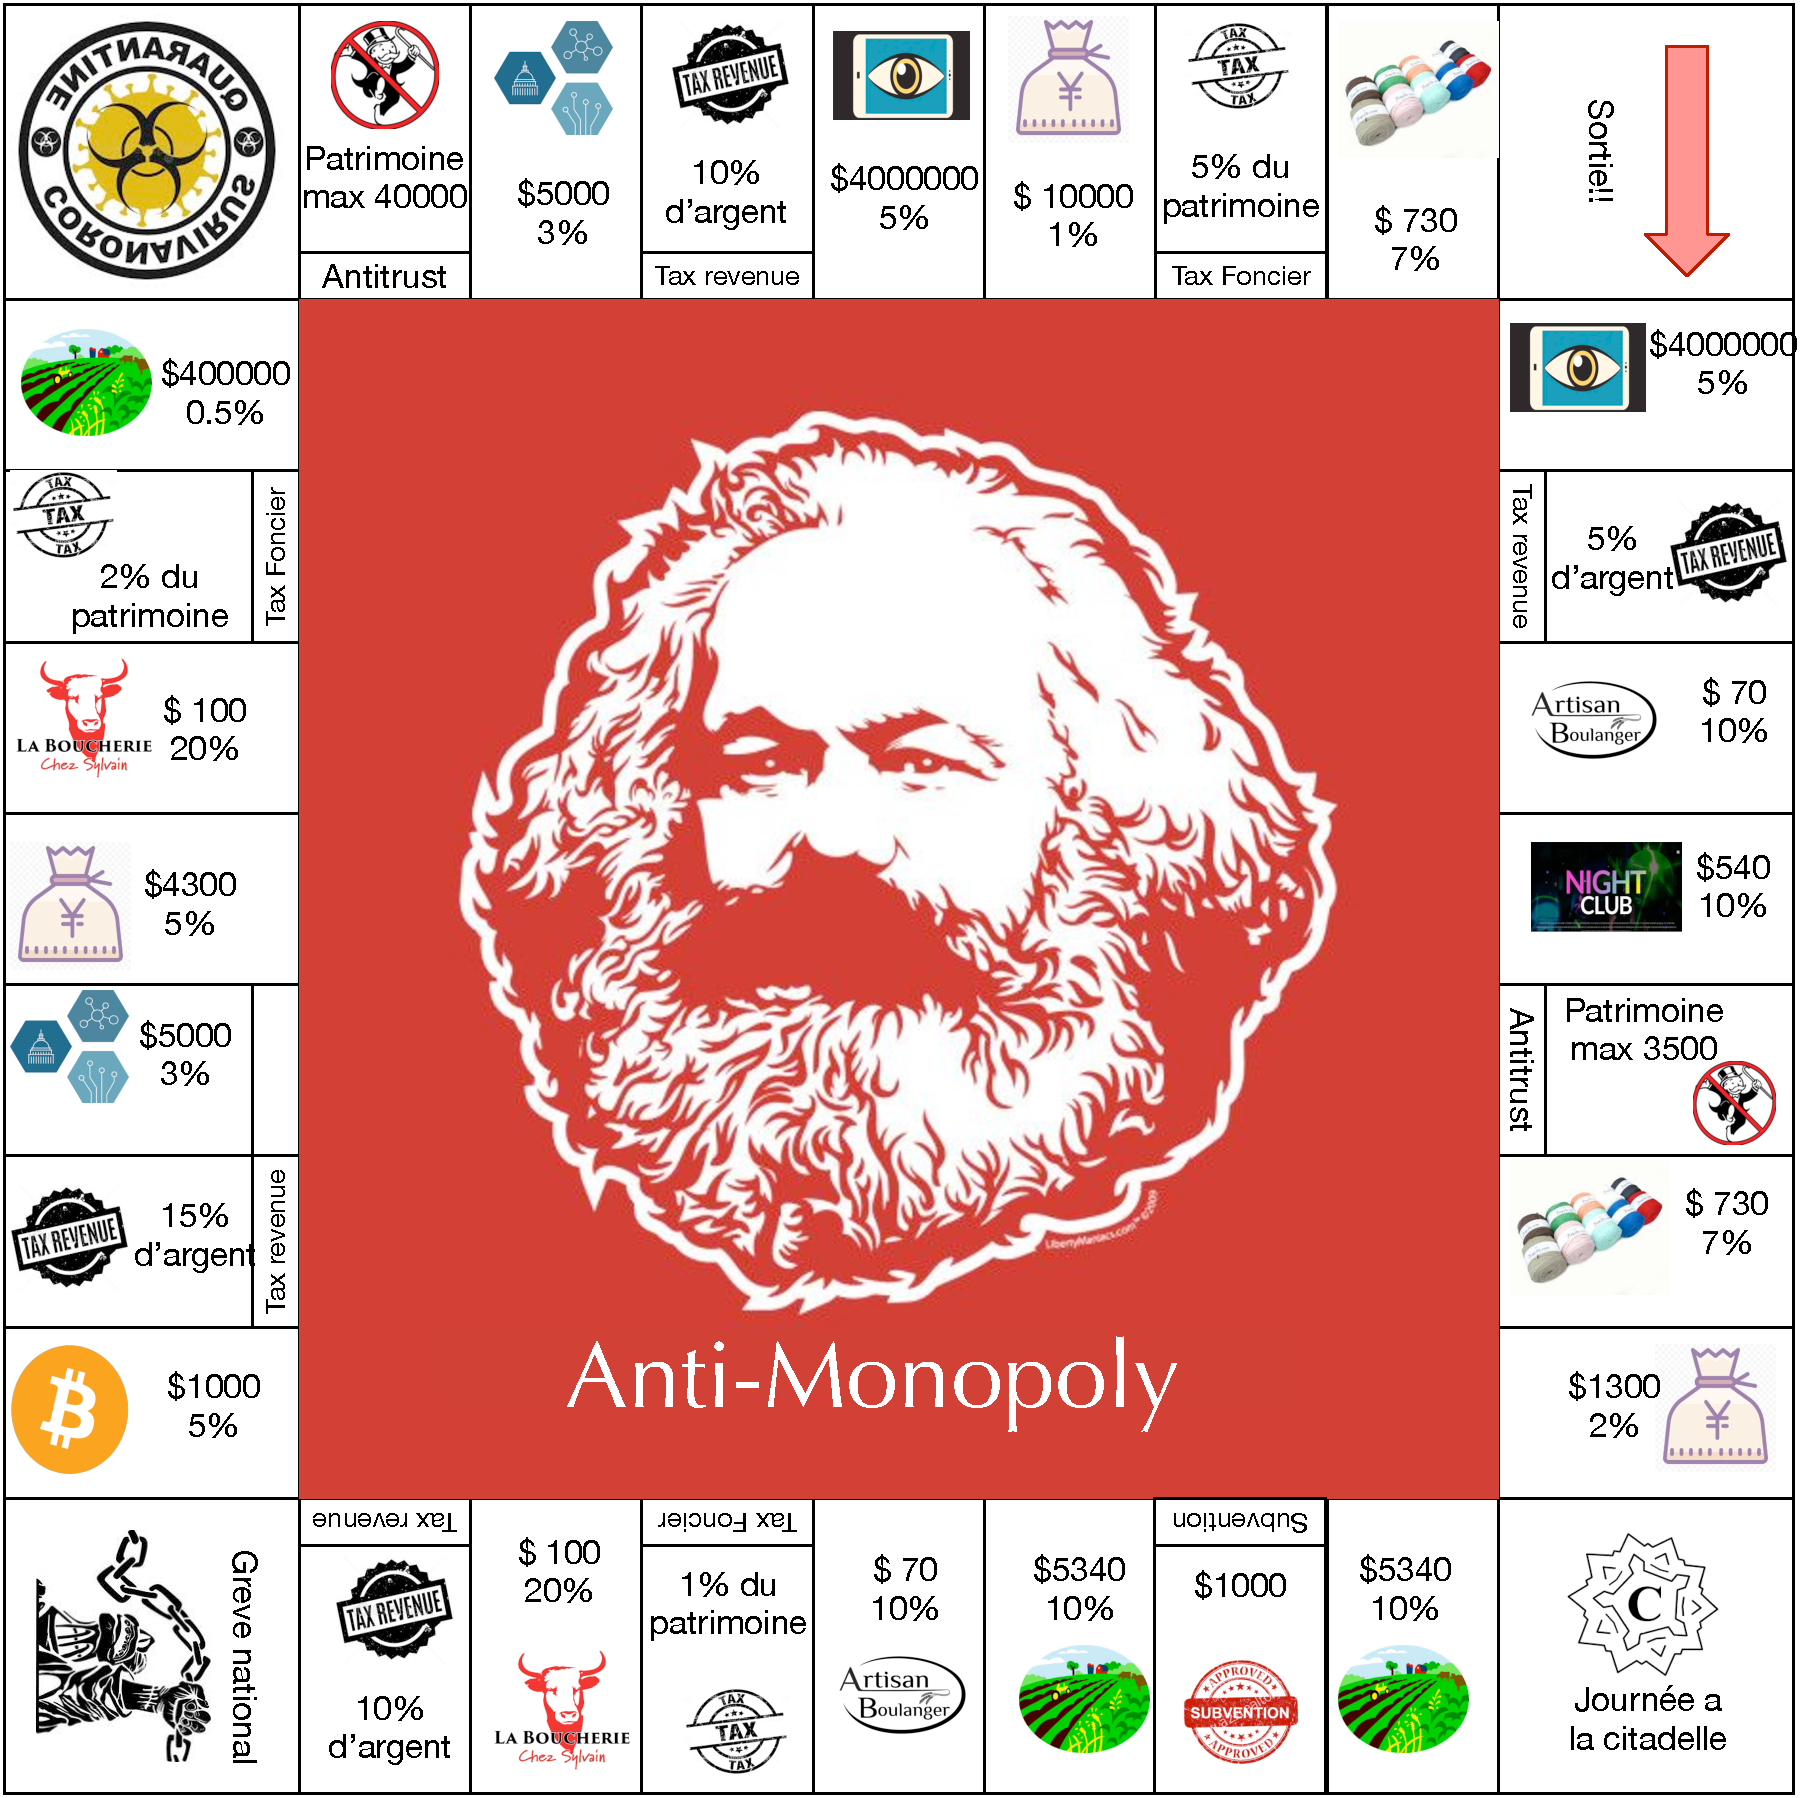
\includegraphics[width=15cm,height=15cm,keepaspectratio]{figures/board.pdf}
\caption{Exemple de tableau de jeu}
\label{fig:tableau}
\end{figure}

	Vous souhaitez implémenter la simulation d'un jeu du style \emph{Monopoly} dans lequel les joueurs cherchent
à augmenter leur patrimoine en marchant sur un chemin où ils doivent prendre des décisions 
d'investissement et faire certaines actions. Attention toutefois à ne pas trop investir, car 
les lois antitrust peuvent vous obliger à distribuer votre richesse.


\section{Caractéristiques du jeu}

    \subsection{Plateau du jeu}
    Le \textbf{plateau} est constitué d'un chemin circulaire composé de \textbf{cases},
dans chacune desquelles il y a des indications. Une case marquée \textbf{sortie}
indique le point de départ du jeu.
	Au moment de construir un plateau, pourrais soit utiliser les configurations dans l'image \autoref{fig:tableau}, ou soit utiliser des configurations inventé pour vous même. 
	En tout case le bout de la construction d'un plateau n'est pas réussir a construire un tableau bien balancé (au sense de jeu), sinon a avoir suffisamment des cases pour pouvoir simuler le jeu.
	
    \subsection{Joueurs}
   
    Il peut y avoir autant de \textbf{joueurs} que souhaité. Chaque joueur a un
montant d'argent initial. Au fur et à mesure que le jeu progresse, chacun des joueurs accroit
ou décroit son argent, selon les décisions d'investissement qu'ils prennent ou d'autres
circonstances. Les capitaux propres d'un joueur correspondent à
son argent plus l'évaluation de tous les investissements qu'il possède.
Si un joueur perd tous ses capitaux il a perdu: il ne peut pas continuer à jouer.
    
    \subsection{L'\'Etat}
    L'\'Etat est un acteur social dont la fonction principale est de réguler l'activité économique des
différents joueurs. Il a des ressources financières. L'État ne participe pas
au jeu en marchant sur le plateau, mais interagit avec tous les joueurs de différentes manières.


    \subsection{La dynamique de jeu}
    Initialement, tous les joueurs sont placés dans la case \textbf{sortie}. 
    
    À tour de rôle, chacun lance
un \textbf{dé} et avance d'où il se trouve d'autant de cases que l'indique le dé. 
    Là, le joueur doit suivre les instructions indiquées dans la case et prend les décisions économiques qu'il juge appropriées.
    
    De cette façon, tous les joueurs avancent à travers le plateau et font leur
entreprise. 
Comme l'itinéraire est circulaire, il n'y a pas de point d'arrivée prédéterminé,
raison pour laquelle ils continuent à tourner jusqu'à la fin du jeu. 
Le jeu a terminé s'il ne reste qu'un seul joueur, si l'État échoue ou ce que l'on souhaite mettre fin au jeu.
En s'agissant d'une simulation, la personne a decider s'on souhaite mettre fin au jeu est l'spectateur de la même.

    
    \subsection{Case}
  
    	Comme on peu voir dans la \autoref{fig:cases}
	  \begin{figure}
    \centering
    \subfigure[]{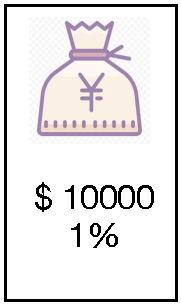
\includegraphics[width=2cm,height=2cm,keepaspectratio]{figures/investissement.pdf}} 
    \subfigure[]{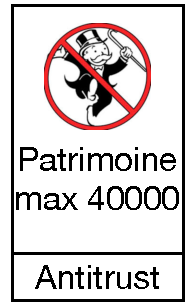
\includegraphics[width=2cm,height=2cm,keepaspectratio]{figures/antitrust.pdf}} 
    \subfigure[]{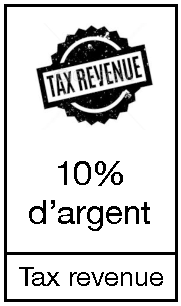
\includegraphics[width=2cm,height=2cm,keepaspectratio]{figures/taxe.pdf}}
       \subfigure[]{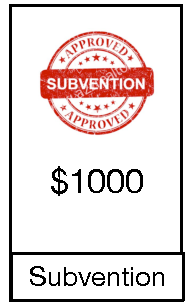
\includegraphics[width=2cm,height=2cm,keepaspectratio]{figures/subvention.pdf}}
      \subfigure[]{
\includegraphics[width=2cm,height=2cm,keepaspectratio]{figures/rienfaire.pdf}}

   
    \caption{(a) Investissment (b) Loi antitrust (c) Finances publiques (d) Subvention (e) Activite non comercial}
    \label{fig:cases}
\end{figure}


        Il existe dans ce jeu différent type de cases. Voici leur particularités:
    \begin{itemize}
        \item \textbf{Investissement}: L'investissement est un cassier que rapport de benefits au propriétaire privé.
        		Chaque investissement compte avec une valeur nominal et un pourcentage que represent l'utilité (ou benefit) de cet investissement. 
		L'investissement a deux états possibles: disponible, et approprié.
		De qu'un joueur arrive a cet case,
		 si l'investissement est possédé par un autre joueur, le joueur arrivant doive payer au propriétaire l'utilité de cet investissement.
		Si par contre, l'investissement est disponible, le joueur décide s'il veut le acheter ou le laissez passer. \footnote{ Plus de détailles sur les investissements dans la prochaine section }
		
	
        \item \textbf{Loi antitrust}: Oblige le joueur à céder tous les investissements
    qu'il possède et qui dépassent le maximum fixé par l'État. 
    Ces investissements reviennent à l'Etat, qui paie le joueur la moitié de leur prix. 

    Exemple, si le maximal d'investissements est 500000 euros, et un joueur a 3 investissements par 200000 (un total de 600000), il doive laisser partir un investissement.  
    Dans la même configuration, si un joueur a 3 investissements par 300000 (un total de 900000), il doive laisser partir deux investissements. 
    Une fois entre les mains de l'état, ces investissements deviennent de nouveau disponibles,  
    en habilitant le future achat. 

        \item  \textbf{Bureau Finances publiques}: Oblige le joueur à payer à l'État un pourcentage de ses
    capitaux propres, au cas où ils dépasseraient une certaine valeur. Chaque taxe se calcule comme un pourcentage du patrimoine du joueur.
    La seule difference entre les types d'impôts, hors du nom, est le pourcentage. 
    Exemples: impôt sur le revenu / 25\% du patrimoine, impôt foncier / 10\% du patrimoine, etc.
        \item \textbf{Subvention}: Le joueur reçoit de l'État le montant indiqué dans la case.
        \item \textbf{Repos}: C'est une case vide dans laquelle rien ne se passe. La \textbf{sortie} en fait partie.
    \end{itemize}
    
    

    \subsection{Investissements}
	Les \textbf{investissements} sont le principal moyen pour les joueurs de gagner de l'argent. 
	Initialement L'\'Etat possède tous les investissements.
	Lorsque un investissement est possédé par l'état, on lui considère \textbf{disponible} pour l'achat. 
	Si par contre le investissement est possédé par un joueur on lui considère \textbf{approprié}.
	
	Chaque investissement a un prix de référence (la valeur nominal),  et un pourcentage d'utilité ou benefit.
	
	Lorsqu'un joueur tombe da une case Investissement, si l'investissement est disponible, cet joueur peut decider de acheter cet investissement. 
	Pour lui acheter il doive payer a l'état la valeur nominal du investissement. 
	
	Lorsqu'un joueur tombe da une case Investissement, si l'investissement est approprié, cet joueur doive payer au propriétaire la valeur d'utilité ce cet investissement. 
	La valuer d'utilité est calculé a partir de la multiplication de la valeur nominal du investissement par le pourcentage de benefit. 
	 
	
    \subsection{Style des joueurs}
    En s'agissant d'une simulation, ou les decisions de joueur sont pris pour le programme, on doive définir des profiles de joueurs.
    Les profiles de joueur proposé sont: \textbf{agressif} et \textbf{prudent}
    
   Chaque type de joueur donc vas prendre decisions différemment  
   
   \paragraph {Le joueur Agressif}  va essayer de tout prendre pour lui le plus vite possible. 
   \begin{itemize}
   	\item En rapport aux investissements: S'il a de l'argent suffisaient,  Il achète tout investissement ou il tombe
	\item En rapport aux loi antitrust: Au moment de choisir qu'investissement se faire exproprier, il prendre les moins chers.
   \end{itemize}
   
  
   \paragraph {Le joueur Prudent}  va de marcher sur de solide, en prennent des decisions un peu plus informées . 
    \begin{itemize}
   	\item En rapport aux investissements: Il ne prendre jamais plus que une quantité configurable maximale des investissements.  Et il n'achète rien plus cher qu'un 20\% de son patrimoine. 
	\item En rapport aux loi antitrust: Au moment de choisir qu'investissement se faire exproprier, il prendre les plus chers.
   \end{itemize}




\section{Simulation}

 Pour jouer ce jeu, on va le faire en mode simulation.
 
 La simulation comprendre trois phases
 
 \begin{description} 
 	\item [Configuration] L'utilisateur configure la simulation
	\item [Jeu] Le jeu démarre. 
	\item [Communication des résultats] On communique les résultats du jeu  
\end{description}
 
 
 \paragraph{La configuration} S'agit du moment ou le joueur doive exprimer que type de simulation est-ce qu'il veut. 
	Avec un de console interactive on va laisser  l'utilisateur définir la quantité des joueurs pour chaque type (Agressif / Prudent), la quantité d'argent a repartir entre les joueurs, la quantité d'argent pour l'État et le profile de simulation. 
 
  Chaque profile de simulation define quel tableau utiliser, comment partager l'argent entre les joueurs, les pourcentages d'impôts, l'argent minimal pour payer impôts , les pourcentages d'utilité des investissements et le patrimoine maximale pour la loi antitrust pour se appliquer. 
  Le joueur doive être capable de choisir entre au moins deux du suivants profiles: 
  \begin{itemize}
  	\item \textbf{NeoLiberal}~: Certains joueurs avec beaucoup d'argent et d'autres avec peu, un état avec quelques
mesures antitrust légères.
  	\item \textbf{Socialiste}~: Tous les joueurs avec le même argent de départ, beaucoup de taxes.
  	\item \textbf{Capitaliste}~: tous les joueurs agressifs, pourcentages de profit élevés, plus élevés
ratio d'investissement.
  	\item \textbf{Progressiste} : plus de joueurs, des lois antitrust strictes
combiné avec des subventions, des pourcentages de profit modérés.
  	\item \textbf{l'Europe après le Covid-19} : (au choix de chacun).
\end{itemize}
 
 
  \paragraph{Le jeu} ou la simulation bien compris. 
  	Une fois on a tout l'information, faire jouer les joueurs une fois par tour de rôle.
	
	 En utilisent la generation des numéros aléatoires pour representer le dé, on doive faire jouer chaque jouer et informer qu'il a fait.
	 
	 Une fois que le tour de rôle est fini (tous les joueurs ont joue) on procède a verifier si le jeu est fini. Si le jeu est fini, on doive sauter a la dernière phase. 
	 
	 Si le jeu n'a pas finit, on doive demander a l'utilisateur s'il veut continuer la simulation. Si oui, on procède au suivant tour de rôle, sinon, on saute a la dernière phase.
	
  
  \paragraph{La Communication des résultats} comprehend la raison du fin de jeu, la declaration du gagnant, l'impression  du ranking des joueurs et l'impression de l'état de l'État. 
  	Par exemple
\begingroup\makeatletter\def\@currenvir{verbatim}
\verbatim
	  l'Etat a échoue! 
	
	  Gagnant Jouer 1 
	  ================
	  	
	   #     Nom            Investissements   Liquide     Patrimoine
	   1 -   Joueur 1       6000              1010        7010
	   1 -   Joueur 2       6000              1010        7010
	   1 -   Joueur 3       6000              1010        7010
	   ==================================================
   Etat - 
        Investissements: 0
        Liquide: 0
\end{verbatim}
   


        
\section{Exigences du projet}

	Sur la base de l'approche générale du jeu, l'implémentation demandée doit comprendre la livraison de:
	
	\begin{description}
		\item [Lundi 1/Juin - 5 Points ] La conception logiciel exprimé en UML au debut d'exercice 
		\item [A livrer a la fin de chaque cours - 3 Points ] Une quantité minimal de 1 tests unitaires par  journée de cours
		\item [Lundi 8/Juin - 2 Points] Point sur l'implementation, revision de la creation du plateau.
		\item [Vendredi 19/Juin - 5 Points]  La conception logiciel exprimé en UML a la fin d'exercice, avec une bref explication de la evolution du modele.
		\item [Lundi 22/Juin - 5 Points] L'implementation complete du simulation 
	\end{description} 
		
	Le cours rendre un maximum de 20 points. 
	Si vous voulez rajouter des points, vous pouvez demander des points bonus.
	


\end{document}

